% beamer loads hyperref and url; let's pass our options to the package
\PassOptionsToPackage{unicode}{hyperref}
\PassOptionsToPackage{hyphens}{url}
\documentclass[
  ignorenonframetext,
  aspectratio=169,
  xcolor={dvipsnames,rgb}
]{beamer}
\usepackage{nus-theme}
\usepackage{jlcode} % from algorithmicx
\usepackage{multirow}
\usepackage{booktabs}

\lstset{
  language=Julia,
  % basicstyle=\small\ttfamily\setbox\strutbox\hbox{},
  basicstyle=\footnotesize\ttfamily,
  showspaces=false,
  showstringspaces=false,
  showtabs=false,
  frame=single,
  breaklines=false,
  breakatwhitespace=false,
  backgroundcolor=\color{white},
  rulecolor=\color{nus@gray},
  aboveskip=1em,
  belowskip=1em,
}

\newcommand{\highlight}[3]{\tikz[baseline=0pt, remember picture,>=stealth] { \node[rounded corners,anchor=base,fill=#1!17] (#2) {#3}; }}
\newcommand{\ubar}[1]{\stackunder[1.2pt]{\(#1\)}{\rule{.8ex}{.075ex}}}

% references
\usepackage[backend=biber, style=lncs]{biblatex}
\addbibresource{references.bib}

% metadata
\hypersetup{
  pdftitle={Extending JumpProcesses.jl for fast point process simulation},
  pdfauthor={Guilherme Augusto Zagatti, Samuel A. Isaacson, Christopher Rackauckas, Vasily Ilin, See-Kiong Ng, Stéphane Bressan},
  pdflang={en},
  hidelinks,
  pdfcreator={Guilherme Zagatti}}

\title{Extending \texttt{JumpProcesses.jl}}
\subtitle{for fast point process simulation}
\author{%
  Guilherme Augusto Zagatti~\inst{1} \and%
  Samuel A. Isaacson~\inst{3} \and%
  Christopher Rackauckas~\inst{4} \and%
  Vasily Ilin~\inst{5} \and%
  See-Kiong Ng~\inst{1,2} \and%
  Stéphane Bressan~\inst{1,2}%
}
\institute{%
  \inst{1} Institute of Data Science, National University of Singapore \and%
  \inst{2} School of Computing, National University of Singapore \and%
  \inst{3} Department of Mathematics and Statistics, Boston University \and%
  \inst{4} Computer Science and AI Laboratory (CSAIL), Massachusetts Institute of Technology \and%
  \inst{5} Department of Mathematics, University of Washington
}
\date[JuliaCon 2023]{\raisebox{-.2\height}{\includegraphics[width=2cm]{logojuliacon.pdf}} \textbf{2023}}

\begin{document}

\begin{frame}
  \titlepage
  % \begin{tikzpicture}[remember picture, overlay]
  %     \node[at=(current page.center),yshift=1.8cm] {};
  % \end{tikzpicture}
\end{frame}

\hypertarget{jump-processes}{\section{Jump processes}\label{jump-processes}}

\begin{frame}{Motivation}

Point processes are a good framework for modelling social interactions.

\begin{figure}
\subfloat[]{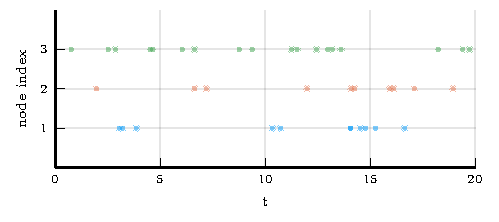
\includegraphics[width=5cm]{assets/hawkes-barcode.pdf}}
\subfloat[]{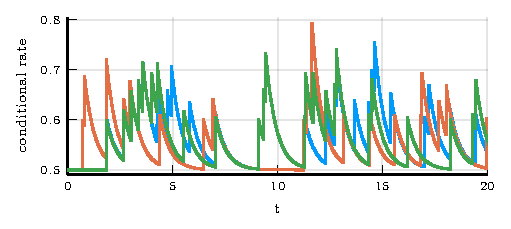
\includegraphics[width=5cm]{assets/hawkes-intensity.pdf}}
\end{figure}

But, \alert{NO} general purpose library for simulating point processes was available!

\end{frame}

\begin{frame}{\texttt{DifferentialEquations.jl}}{Suite for numerically solving \( u \)}

\vspace{2em}

{\Large
\[
  du = 
      f(u, p, t) \eqnmarkbox[nus@gray]{deterministic}{dt} 
    + g (u, p, t) \eqnmarkbox[nus@orangebright]{diffusion}{dW (t)} 
    + h (u, p, t) \eqnmarkbox[nus@bluebright]{jump}{dN (t)}
\]
}

\annotate[yshift=1em]{above,left}{deterministic}{\textbf{Deterministic component}}
\annotate[yshift=0.75em]{above}{diffusion}{\textbf{Diffusion component}\\``some change occurs during any\\time interval, however small, but in small\\time intervals the changes are small''\\\citet{feller1949}}
\annotate[yshift=-1.5em]{below,left}{jump}{\textbf{Jump component}\\``the system remains for a time unchanged,\\then undergoes a sudden change into another state.'' \citet{feller1949}}

\vspace{3em}

\alert{\texttt{JumpProcesses.jl}} Core library of \texttt{DifferentialEquations.jl} to sample the jump component.

Lacked efficient methods to simulate jumps with locally-bounded variable intensity rates.

\end{frame}

% Don’t forget that your audience will likely not know much about jump processes in general, so a bit of an introduction to them and what they can be used for (and what the problem CoEvolve solves is) will likely be very helpful.

\begin{frame}{Jump (or point) process}

\fullsizegraphic{svg-inkscape/simple-jump.pdf}

Models the occurrence of random points (or events) over a support. 

\vspace{3em}

\begin{description}[labelwidth=2cm]
  \item[Seismology] Epidemic type after-shock (ETAS) model, \eg~\citet{saichev2007}
  \item[Neuroscience] Model of hippocampal synaptic plasticity, \eg~\citet{rodrigues2021}
  \item[Finance] Asset price and financial risk models, \eg~\citet{bjork2021}
  \item[Biochemistry] Well-stirred chemically reacting systems, \eg~\citet{gillespie2001}
  \item[Social Media] Information diffusion and social network evolution, \eg~\citet{farajtabar2017}
\end{description}

\end{frame}

\begin{frame}{Jump processes are point processes}

\fullsizegraphic{svg-inkscape/jump-as-measure.pdf}

\( N (t) \) denotes the total number of jumps over \( [0, t] \), we assume no common jumps:
\[
  P(N(t + dt) - N(t) \in \{ 0, 1 \}) = P( dN(t) \in \{ 0, 1 \}) = 1
\]

\vspace{5em}

\( N[t_1, t_2] \) denotes the total number of points in \( [t_1, t_2] \). 

\vspace{1em}

In other words, \( N( \cdot ) \) is a random integer measure of the positive real line. 

\end{frame}

% \begin{frame}{Constructing jump intervals}

% \fullsizegraphic{svg-inkscape/prob-intervals.pdf}

% \vspace{-2em}

% Most jump processes over a temporal support can be described according to the likelihood that jumps appear over time.

% \vspace{10em}

% The diagram presents two manners of constructing a jump processes, either via the {\color{nus@bluebright} interarrival} or {\color{nus@orangebright} waiting} interval.

% \end{frame}

\begin{frame}{Conditional intensity}

Evolutionary or temporal processes are jump processes over a uni-dimensional support, their likelihhod is fully characterized by its conditional intensity --- itself a stochastic process:

\vspace{2em}

\[
  \lambda^{\eqnmarkbox[nus@gray]{conditioning}{\ast}} (t) \equiv \lambda(t \mid \eqnmarkbox[nus@gray]{history}{H_{t^-}}) = 
    \frac{
      \eqnmarkbox[nus@orangebright]{pdf}{p^\ast(t)}
    }{
      \eqnmarkbox[nus@bluebright]{survival}{1 - \int_{t_n}^{t} p^\ast(u) \, du}
    }
\]

\annotate[yshift=1.5em]{above,left}{history,conditioning}{History of events, \( H_{t^-} = \{ (t_n, k_n) \mid 0 \leq t_n \leq t \}\)\\\( \ast \) denotes the conditioning on \( H_{t^-} \)}
\annotate[yshift=1em]{above,right}{pdf}{Prob.\@ density of event taking place\\at time \( t \) given \( H_t \)}
\annotate[yshift=-1em]{below,left}{survival}{Survival function,\\no event takes place from \( t_n \) until \( t \)}

\vspace{4em}

It can be interpreted as the rate of event per unit of time: \( E(dN(t) \mid H_{t^-}) \approx \lambda^\ast(t) \; dt \). 

\end{frame}

\begin{frame}{Compensator}

The compensator is the sum of the conditional intensity over time.
\[
  \Lambda^\ast (t_n) \equiv \tilde{t}_n \equiv \int_0^{t_n} \lambda^\ast (u) du
\]
The transformed data \( \tilde{t}_n \) forms a homogeneous Poisson process with unit rate.
\[
  \Delta \tilde{t}_n \equiv \tilde{t}_n - \tilde{t}_{n-1} \sim \exp(1)
\]

\end{frame}

\begin{frame}{Contribution}

\fullsizegraphic{svg-inkscape/contribution.pdf}

\vspace{-3em}

We extended \texttt{JumpProcesses.jl} with a new simulation algorithm, \texttt{Coevolve}, that enables the rapid simulation of processes with a non-negative, left-continuous, history-adapted and locally bounded intensity rate coupled or not with differential equations such as the one below.

\vspace{5em}

One of the few readily available, fast, general-purpose libraries for simulating temporal point processes.

\end{frame}

\begin{frame}{Three techniques for simulating a jump process}

\begin{description}

  \item[Inverse] Draw successive realizations from \( \Delta \tilde{t}_n \sim exp(1) \) and solve \( \Delta \tilde{t}_n = \int_{t_{n-1}}^{t_n} \lambda^\ast (u) du \) for \( t_n \, \).

  \item[Thinning] Successively sample a homogeneous processes, then thin the obtained points with the conditional intensity of the original process.

  \item[Queuing] Use a priority queue to determine the order in which events occur; update the queue after each event takes place.

\end{description}

\end{frame}

\begin{frame}[fragile=singleslide]{Simple simulation using \texttt{JumpProcesses.jl}}

\[
  du = d N(t) \qquad \lambda^\ast (t) = 0.25
\]


\begin{lstlisting}
  # re-exports DiffEqBase
  using JumpProcesses
  rate(u, p, t) = p[1]
  affect!(integrator) = integrator.u[1] += 1
  jump = ConstantRateJump(rate, affect!)
  u, tspan, p = [0.], (0., 200.), (0.25,)
  # holds general problem parameters
  dprob = DiscreteProblem(u, tspan, p)
  # holds jump parameters
  jprob = JumpProblem(dprob, Coevolve(), jump; dep_graph=[[1]])
  # solves jump problem with given stepper
  sol = solve(jprob, SSAStepper())
\end{lstlisting}

\end{frame}

\hypertarget{benchmarks}{\section{Benchmarks}\label{benchmarks}}

\begin{frame}{Benchmark Setup}

All benchmarks available in \texttt{SciMLBenchmarks.jl} and run with BuildKite via the continuous integration facilities provided by the package maintainers.

\vspace{2em}

Two sets of benchmarks: (1) systems containing only \texttt{ConstantRateJump} and (2) general systems containing any type of temporal jump.

\vspace{2em}

Added two benchmark suites to assess the performance of the new aggregators under settings that could not be previously simulated.

\end{frame}

\begin{frame}[fragile=singleslide]{The compound Hawkes process}{A mutually exciting process}

\vspace{-1em}

\begin{columns}

\column[t]{0.5\textwidth}

\[
  \lambda_i^\ast (t) = \lambda + \sum_{j \in E_i} \sum_{t_{n_j} < t} \alpha \exp \left[-\beta (t - t_{n_j}) \right]
\]

Recursively, it simplifies to:

\begin{alignat*}{3}
  &\lambda_i^\ast (t)      & = & \, \lambda + \phi_i^\ast (t) \\
  &\phi_i^\ast (t)         & = & \, \exp \left[ -\beta (t - t_{N_i}) \right] \left( \alpha + \phi_i^\ast (t_{N_i}) \right) \\
  &\phi_i^\ast(t_{0_i}) \, & = & \, 0
\end{alignat*}

\column[t]{0.5\textwidth}

\begin{lstlisting}[basicstyle=\scriptsize\ttfamily,escapechar=\#]
function rate(u, p, t)
    #λ#, #α#, #β#, h, urate, #ϕ# = p
    urate[i] = #λ# + exp(-#β# * (t - h[i])) * #ϕ#[i]
    urate[i]
end

function affect(integrator)
    #λ#, #α#, #β#, h, urate, #ϕ# = integrator.p
    for j in g[i]
        #ϕ#[j] *= exp(-#β# * (integrator.t - h[j]))
        #ϕ#[j] += #α#
        h[j] = integrator.t
    end
    integrator.u[i] += 1
end
\end{lstlisting}
  
\end{columns}

\end{frame}

\begin{frame}{The compound Hawkes process benchmark}{Simulation of 10-nodes compound Hawkes process}

\fullsizegraphic{svg-inkscape/hawkes.pdf}

\vspace{2em}

\begin{figure}
\subfloat[]{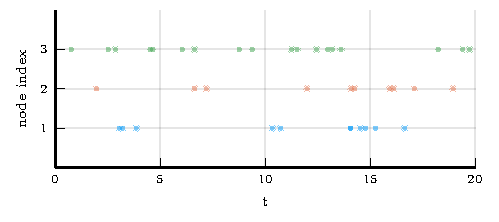
\includegraphics[width=5cm]{assets/hawkes-barcode.pdf}}
\subfloat[]{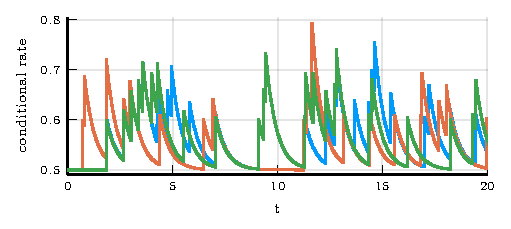
\includegraphics[width=5cm]{assets/hawkes-intensity.pdf}}
\subfloat[]{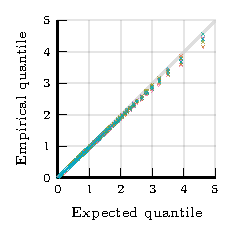
\includegraphics[width=3cm]{assets/hawkes-qqplot.pdf}}
\end{figure}


\end{frame}

\begin{frame}{NEW BENCHMARK The compound Hawkes process}{Median execution time, 50 samples per node (V) x time}

\begin{tikzpicture}

  \node[anchor=south west] (image) at (0, 0) {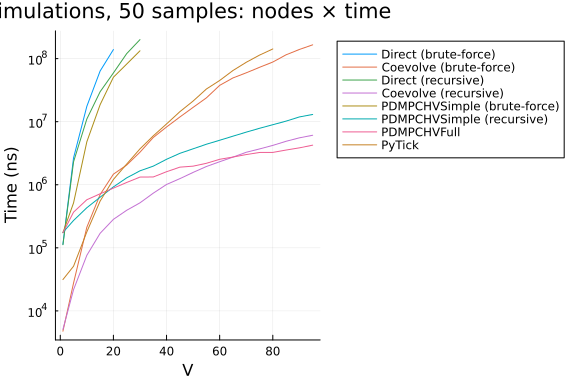
\includegraphics[trim={0 0 0 0.8cm},clip,width=10cm]{assets/hawkes-benchmark.png}};
  \node[text width=8cm,overlay,yshift=3.5cm,xshift=-4.5cm,anchor=north west] at (image.south east) {%
    \footnotesize\textit{brue-force} loops through the whole history of past events. \textit{recursive} only looks at the previous state of each node.};

\end{tikzpicture}

\end{frame}

\begin{frame}{NEW BENCHMARK Synapse}{Median execution time and memory allocation, 50 samples}

\begin{columns}

  \column{0.5\textwidth}

  \begin{table}
  \centering
  \begin{tabular}{lll} 
  \toprule
   & \textbf{Time} & \textbf{Allocation}  \\ 
  \hline
  \textbf{\textit{Inverse}} & -  & - \\ 
  \textbf{\texttt{Coevolve}} & \underline{4.9 s} & \underline{95.2 Mb}  \\
  \textbf{\textit{CHV}} & \textbf{2.4 s} & \textbf{43.8 Mb} \\
  \bottomrule
  \end{tabular}
  \end{table}

  \column{0.5\textwidth}

  Stochastic model of hippocampal synaptic plasticity with geometrical readout of enzyme dynamics proposed in \citet{rodrigues2021}.

  \vspace{.5em}

  System with 98 jumps affecting 49 discrete variables and a stiff, ODE problem containing 34 continuous variables which affect jump rates.

  \vspace{.5em}

  \texttt{Coevolve} lags due to large rejection rate (\( \approx 70\% \)) of the thinning procedure leading to 2-3 \(\times\) more function evaluations and Jacobians created.

\end{columns}

\end{frame}

\begin{frame}{\texttt{ConstantRateJump} benchmarks}{Median execution time}

\begin{table}
\centering
\begin{tabular}{lccccc}
\toprule
 & \multicolumn{1}{c}{\textbf{ Diffusion }} & \multicolumn{1}{c}{\textbf{ Multi-state }} & \multicolumn{1}{c}{\textbf{ Gene I }} & \multicolumn{1}{c}{\textbf{ Gene II }} \\
\hline
\textbf{\texttt{Direct}}         & 7.18 s             & 0.16 s             & \underline{0.24 ms} & \underline{0.59 s} \\
\textbf{\texttt{FRM}}            & 15.04 s            & 0.25 s             & 0.29 ms             & 0.78 s             \\
\textbf{\texttt{SortingDirect}}  & 1.08 s             & \underline{0.11 s} & \textbf{0.23 ms}    & \textbf{0.50 s}    \\
\textbf{\texttt{NRM}}            & 0.75 s             & 0.25 s             & 0.39 ms             & 0.89 s             \\
\textbf{\texttt{DirectCR}}       & \underline{0.51 s} & 0.21 s             & 0.47 ms             & 1.00 s             \\
\textbf{\texttt{RSSA}}           & 1.42 s             & \textbf{0.10 s}    & 0.43 ms             & 0.65 s             \\
\textbf{\texttt{RSSACR}}         & \textbf{0.46 s}    & 0.16 s             & 0.91 ms             & 1.07 s             \\
\textbf{\texttt{Coevolve}}       & 0.90 s             & 0.36 s             & 0.59 ms             & 1.33 s             \\
\bottomrule
\end{tabular}
\caption{A 1-dimensional continuous time random walk approximation of a diffusion model (Diffusion), the multi-state model from Appendix A.6~\citet{marchetti2017} (Multi-state), a simple negative feedback gene expression model (Gene I) and the negative feedback gene expression from~\citet{gupta2018} (Gene II). Fastest time is \textbf{bold}, second fastest \underline{underlined}.}
\end{table}

\end{frame}

\hypertarget{jumpprocesses.jl}{\section{JumpProcesses.jl}\label{jumpprocesses.jl}}

\begin{frame}[fragile=singleslide]{\texttt{DifferentialEquations.jl} callbacks}

We solve differential equations by taking small steps \( dt \), but jumps occurs at large, arbitrary steps.

\texttt{DifferentialEquations.jl} provides callbacks to add arbitrary breakpoints in the stepper.

\begin{lstlisting}
  using DiffEqBase
  # condition(u, t, integrator), when the callback should be used
  # affect!(integrator), modifies the integrator
  DiscreteCallback(condition, affect!)
\end{lstlisting}

\end{frame}

\begin{frame}[fragile=singleslide]{\texttt{AbstractSSAJumpAggregator}}{A custom \texttt{DifferentialEquations.jl} callback}

\texttt{JumpProcesses.jl} is a wrapper around the callback facility that allow us to sample jumps according to the conditional intensity \( \lambda^\ast (t) \).

Except for the inverse method, all the algorithms for simulating temporal jump processes are based on \texttt{AbstractSSAJumpAggregator}:

\begin{lstlisting}
# JumpProcesse.jl/src/aggregators/ssajump.jl
function DiscreteCallback(c::AbstractSSAJumpAggregator)
    DiscreteCallback(c, c, initialize = c,
      save_positions = c.save_positions)
end
\end{lstlisting}

\end{frame}

\begin{frame}[fragile=singleslide]{Overloading \texttt{AbstractSSAJumpAggregator}}

\texttt{condition(u, t, integrator)}

\begin{lstlisting}
function (p::AbstractSSAJumpAggregator)(u, t, integrator)
    p.next_jump_time == t
end
\end{lstlisting}

\texttt{affect!(integrator)}: Most of the action is in here!

\begin{lstlisting}
function (p::AbstractSSAJumpAggregator)(integrator::I)
  execute_jumps!(p, integrator, integrator.u, integrator.p,
      integrator.t, p.affects!)
  generate_jumps!(p, integrator, integrator.u, integrator.p,
      integrator.t)
  register_next_jump_time!(integrator, p, integrator.t) 
  nothing
end
\end{lstlisting}

\end{frame}

\begin{frame}[fragile=singleslide]{\texttt{DifferentialEquations.jl} steppers}

Steppers determines the \alert{evolution} from \texttt{tspan[1]} to \texttt{tspan[2]} in terms of discrete steps and the rules for updating the integrator at each step.

\begin{lstlisting}
# generic solver (not actual implementation)
function solve!(integrator)
  preamble!(integrator)
  while should_continue_solve(integrator) # depends on t and tstop
      loopheader!(integrator)
      step!(integrator)
      loopfooter!(integrator) # handle callbacks
  end
  postamble!(integrator)
end
\end{lstlisting}

\end{frame}

\begin{frame}[fragile=singleslide]{\texttt{SSAStepper}}{A custom \texttt{DifferentialEquations.jl} stepper}

Callbacks are called at every step, but steppers are not guaranteed to stop at time positions when the callback condition is true \alert{unless} these are assigned to \texttt{integrator.tstop}.

\texttt{JumpProcesses.jl} defines own stepper \texttt{SSAStepper} to handle jump-only problems \( du = h (u, p, t) dN (t) \).

\begin{lstlisting}
function register_next_jump_time!(integrator::SSAIntegrator,
    p::AbstractSSAJumpAggregator, t)
    integrator.tstop = p.next_jump_time
    nothing
end
\end{lstlisting}
\end{frame}

\begin{frame}[fragile=singleslide]{\texttt{SSAStepper}}{A custom \texttt{DifferentialEquations.jl} stepper}

Generic integrators can also handle \texttt{AbstractSSAJumpAggregator}, but less efficiently.

\begin{lstlisting}
function register_next_jump_time!(integrator,
    p::AbstractSSAJumpAggregator, t)
    if p.next_jump_time < p.end_time
        add_tstop!(integrator, p.next_jump_time)
    end
    nothing
end
\end{lstlisting}

\end{frame}

\begin{frame}[fragile=singleslide]{Aggregator types}

\begin{lstlisting}[escapechar=\#,frame=tblr]
    jprob = JumpProblem(prob, #\highlight{nus@bluebright}{aggregator}{aggregator}#, #\highlight{nus@bluebright}{jumps}{jumps}#; #\highlight{nus@orangebright}{depgraph}{dep\_graph}#)
\end{lstlisting}

\begin{tikzpicture}[remember picture,overlay,>=stealth,nodes={align=left,inner ysep=1pt}]
  \node[color=nus@bluebright!85,yshift=1.1cm] (aggregatortext) at ($(aggregator.south)!0.5!(jumps.south)$) {%
    \textsf{\footnotesize The wrapper initializes the \texttt{aggregator<:AbstractAggregatorAlgorithm} with the listed jumps.}};
  \draw [<-,color=nus@bluebright] (aggregator.north) |- (aggregatortext.south) -| (jumps.north);
  \node[anchor=east,color=nus@orangebright!85,yshift=-0.8cm] (depgraphtext) at (depgraph.south) {%
    \textsf{\footnotesize Required for some aggregators.}};
  \draw[color=nus@orangebright] (depgraph.south) |- ([xshift=-0.3ex, yshift=-0.2ex]depgraphtext.south west);
\end{tikzpicture}

\begin{description}

  \item[Inverse] Not available

  \item[Thinning] \texttt{Direct}, \texttt{DirectFW}, \texttt{DirectCR}, \texttt{SortingDirect}, \texttt{RDirect}, \texttt{RSSA}, \texttt{RSSACR}
    
  \item[Queuing] \texttt{FRM}, \texttt{FRMFW}, \texttt{NRM}, \texttt{Coevolve}

\end{description}

\end{frame}

\begin{frame}[fragile=singleslide]{Two different types of jumps}

\begin{description}

  \item[\texttt{ConstantRateJump(rate, affect!)}] The conditional intensity is constant between jumps, \ie \( \lambda^\ast(t) = \lambda_n^\ast \) which can be handled by any aggregator. 

  Note that the API also includes \alert{\texttt{MassActionJump}} which is a special case to simulate systems that can be represented in mass action form.

  \item[\texttt{VariableRateJump(rate, affect!; urate, rateinterval, lrate)}] The conditional intensity can vary between jumps. It can only be handled by the inverse method.

  When it is locally bounded, it can also be handled by the Coevolve aggregator, \ie let \( \bar{B}^\ast (t) = \bar{B}(t \mid H_t) \), \( \ubar{B}^\ast (t) = \ubar{B}(t\mid H_t) \) and \( L^\ast(t) = L(t \mid H_t) \) such that \( \lambda^\ast \, (t + u)  \leq \bar{B}^\ast(t) \)  and \( \lambda^\ast \, (t + u)  \geq \ubar{B}^\ast(t) \) for all \( 0 \leq u \leq L^\ast(t) \).

\end{description}

\end{frame}

\begin{frame}{Thinning}

\fullsizegraphic{svg-inkscape/thinning-general.pdf}

\end{frame}

\begin{frame}{Thinning constant rates}

\fullsizegraphic{svg-inkscape/thinning-constant.pdf}

\end{frame}

\begin{frame}{Queuing}{The \texttt{Coevolve} approach}

\fullsizegraphic{svg-inkscape/queueing.pdf}

\end{frame}

\hypertarget{conclusion}{\section{Conclusion}\label{conclusion}}

\begin{frame}{Conclusion}

\texttt{JumpProcesses.jl} is a fast, general-purpose library for simulating temporal point processes. 

With the addition of \texttt{Coevolve}, any point process on the real line with a non-negative, left-continuous, history-adapted and locally bounded intensity rate can be simulated.

Way forward:

\begin{itemize}

  \item Include \textit{CHV} as a new aggregator for \texttt{VariableRateJump} \textit{WIP}

  \item Automatic selection of bounds using automatic differentiation?

  \item More inexact methods and compound branching processes?

  \item N-dimensional jumps?

\end{itemize}

\end{frame}

\begin{frame}
  \thispagestyle{empty@titlepage}
  \begingroup
    \setbeamercolor{structure}{fg=white}
    \begin{beamercolorbox}[sep=8pt,center]{title}%
      {\usebeamerfont{title}\usebeamercolor{title}Thank you!}%
      \vskip1em%
      {\usebeamerfont{subtitle}\usebeamercolor[fg]{subtitle}\href{https://gzagatti.org}{gzagatti.org}}%
    \end{beamercolorbox}
  \endgroup
\end{frame}

\begin{frame}[t,allowframebreaks]
  \frametitle{References}
  \printbibliography[heading=none]
\end{frame}

\end{document}
